\subsubsection{Key - Online} \label{section:counter-replace-encryption-key-online}
An idea to handle the encryption key is to store it on a server and provide it to the application.
This works similar to the license verification.
When the decryption inside the application is called, the user is verified on the server.
In case the check is successful, the decryption key is send to the device.
The advantage over having the original implementation is to have an unguessable result.
The key can either be retrieved from the server for each decryption action or it can be cached on the device.
Caching should be favored since getting the key for each action requires to be online, it slows down the application and it generates additional traffic.
In order to improve security, keys can be changed when updating the version of the application.
\begin{figure}[h]
    \centering
    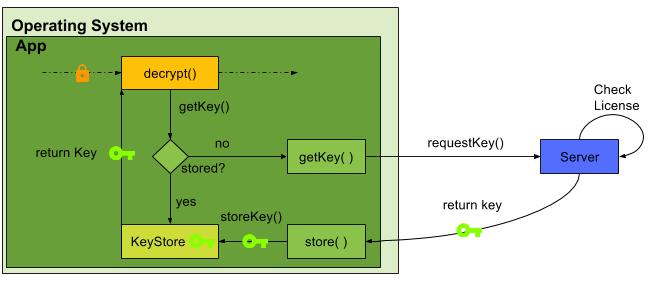
\includegraphics[width=0.8\textwidth]{data/encryptionKeyServer.png}
    \caption{Retrieving the key after successful identification from the server and store it local on device}
    \label{fig:encryptionKeyServer}
\end{figure}
